
%(BEGIN_QUESTION)
% Copyright 2014, Tony R. Kuphaldt, released under the Creative Commons Attribution License (v 1.0)
% This means you may do almost anything with this work of mine, so long as you give me proper credit

I dette fasordiagrammet, avgjør hvilken fasor som {\it leder} og hvilken som {\it henger etter} den andre:

$$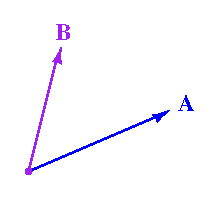
\includegraphics[width=15.5cm]{i00840x01.eps}$$

\underbar{file i00840}
%(END_QUESTION)





%(BEGIN_ANSWER)

I dette diagrammet leder fasor ${\bf B}$ fasor ${\bf A}$. Etter konvensjon roterer fasorer normalt mot klokken. Hvis du ser for deg at pilspissene på disse fasorene er to racerbiler som kjører i ring, er bilen som ligger foran den {\it ledende}, mens bilen bak er den {\it hengende etter}.

%(END_ANSWER)





%(BEGIN_NOTES)


%INDEX% Electronics review, phasor expressions of circuit quantities

%(END_NOTES)
